\mysection{トルクコンバータの概要}
トルクコンバータとは流体のエネルギーを利用してトルクの変換を行うものである。
図\ref{im1}にトルクコンバータの基本構造と作動原理を示す。
入力側に結合された\textbf{\textgt{ポンプ羽根車}}、出力側に結合された\textbf{\textgt{タービン羽根車}}、ケースに固定された\textbf{\textgt{ステータ}}から成る。
内部に作動流体として油が充満されていて、入力側と出力側の回転差によりトルクの増幅作用が発生する。
これらにより、\textbf{\textgt{機械エネルギー}}を一度\textbf{\textgt{流体エネルギー}}に変換し、再度\textbf{\textgt{機械エネルギー}}に変換することで、動力を伝達する仕組みを構成する。

\mysubsection{原理}
ポンプ羽根車がエンジンによって駆動する。その後、内部の流体が羽に沿って外方向に押し出され、
図\ref{im1}の矢印の方向に流れてタービンに流入する。
この流体の運動エネルギーによってタービンにトルクを与えて回転させる。
最後にステータを通って再びポンプに流入する。

\begin{figure}[H]
  \begin{center}
  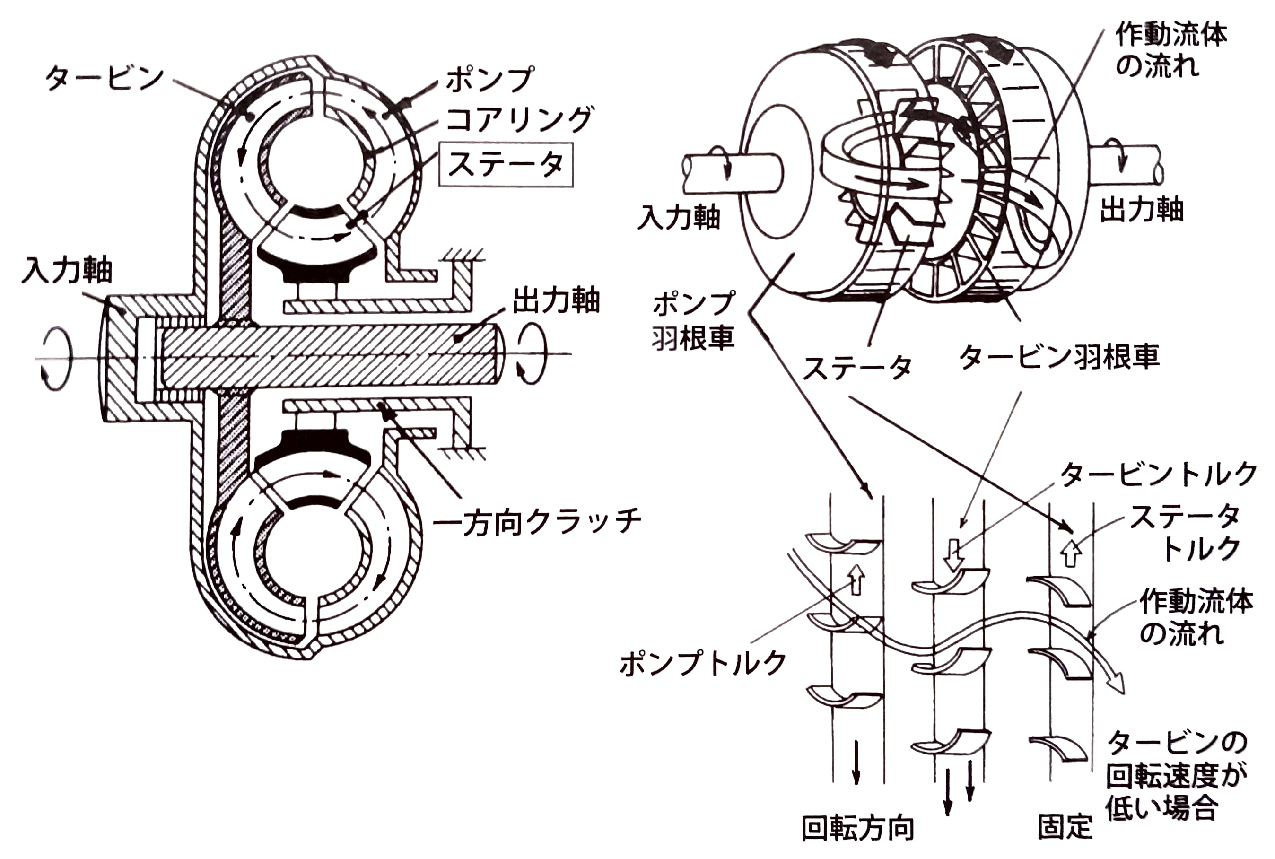
\includegraphics[width=.38\columnwidth]{img/1_en2_1.pdf}
  \caption{トルクコンバータの基本構造と作動原理}
  \label{im1}
  \end{center}
\end{figure}

\mysubsection{技術水準}
トルク比の上昇、効率の向上、異なる特性を得るために、様々な種類・型式が提案されている。
トルクコンバータは、\textbf{\textgt{要素・段・相}}によって分類される。要素は、羽根車の総数を表す。
段はポンプとタービンの組み合わせの段である。
相は、ステータの固定・空転により、特性が2通りに変化する特性の運転範囲の数を表す。
ステータは一方向クラッチで出力軸の回転方向に回転し、逆方向には固定される。
このクラッチ点を境に特性が変化する。したがってクラッチ点が1つの時はその前後で2相、クラッチ点が2つの時は3相となる。
図\ref{im2}に自動車用のトルクコンバータの型式例を示す。現在の自動車用自動変速機には3要素1段2相型トルクコンバータが多く使用されている。

\begin{figure}[H]
  \begin{center}
  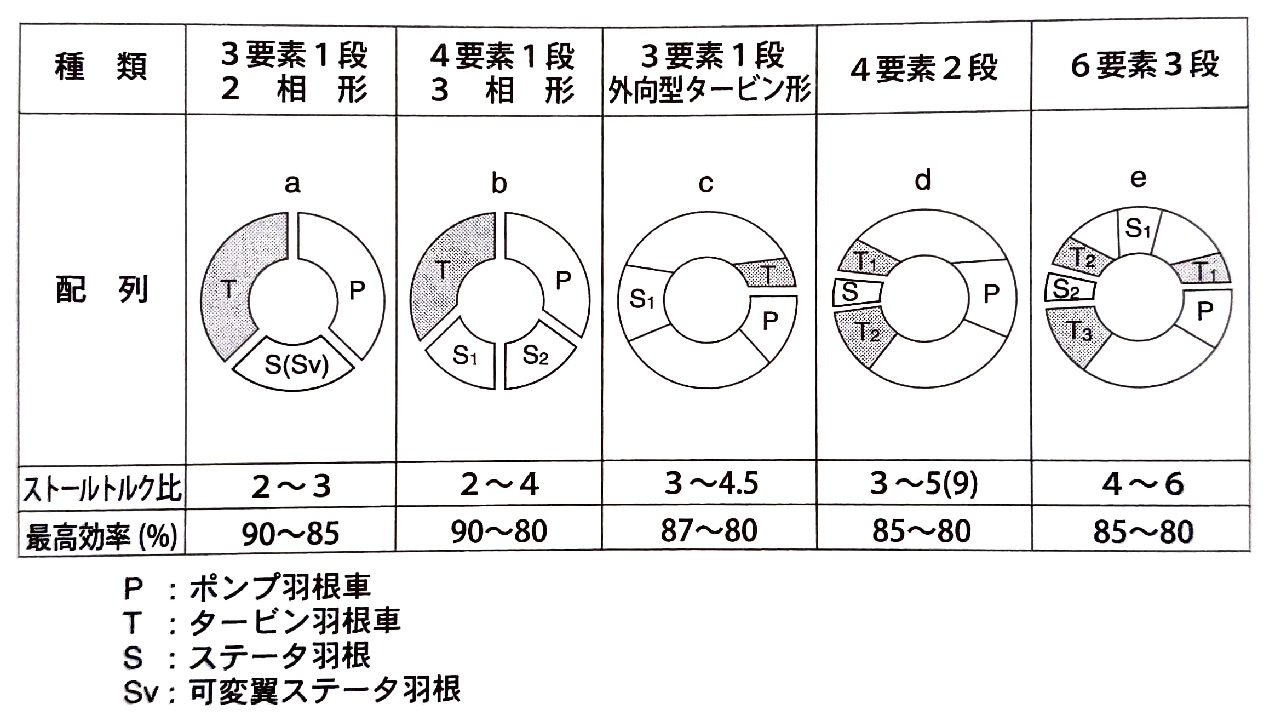
\includegraphics[width=.4\columnwidth]{img/3_en2_1.pdf}
  \caption{自動車用トルクコンバータの型式模型}
  \label{im2}
  \end{center}
\end{figure}

\vspace{-5mm}
\mysection{社会的な背景}
\vspace{5mm}
\mysubsection{歴史的な背景}
1905年、ドイツの\textbf{\textgt{ヘルマン・フェッティンガー}}がトルクコンバータの原型となる装置を発明した。
船舶用に開発されたもので、減速機構でトルクを高める効果を備えていた。
その後、1920年代の後期から1930年代にわたって、始動の容易性、トルク変換性、
自動変速性などの特長を活かすため、自動車の動力伝達装置への適用が検討された。
具体的には、1.車両発進時のけん引力増加のための低速度比におけるトルク比を大きくするための\textbf{\textgt{多段化}}、
2.車両の定常走行時の経済性向上のための高速度比における効率を高めることのために、\textbf{\textgt{機械式直結装置の付加}}、\textbf{\textgt{トルクコンバータと流体継手の一体化}}が行われた。
現在に至るまで、多段化と変速機と流体継手の組み合わせの試行によって、トルクコンバータの性能向上が図られている。

\mysubsection{環境負荷}
1970年代まで、トルクコンバータの作動流体として\textbf{\textgt{鯨油}}が使われていた。
鯨油は、\textbf{\textgt{高温で化学反応が鈍くなる}}欠点がある。
そのため1970年代以降の\textbf{\textgt{排ガス規制}}と\textbf{\textgt{燃費対策}}のための需要(エンジン冷却水の温度を高く保つ)に不向きとなった。
さらに、\textbf{\textgt{商業捕鯨}}の規制により継続生産が困難となったため、化学合成剤に代替された。

\mysubsection{経済性}
自動車用において、トルクコンバータは変速機構ギアセットと組み合わせて、
ステップATとして使われていたが、\textbf{\textgt{動力の伝達ロスが大きいため燃費が悪い}}という欠点がある。
そのため、伝達ロスの少ない方式として、プーリーを介してベルトで接続する形式のCVTや、
奇数段ギアと偶数段ギアそれぞれにクラッチが装備されMTと同じく物理的にクラッチがつながるDCTのAT車の割合が一時期に増加した。

\mysubsection{技術水準}
\textbf{\textgt{電子制御の進化}}によって、自動車用トルクコンバータの伝達ロスのデメリットが改善された。
伝達ロスを軽減する方法として、エンジンとトランスミッションを直結させる\textbf{\textgt{ロックアップ機構}}という方法がある。
しかし、CVTやDCTなみに伝達ロスを軽減するには精度の高い制御が必要だった。
その後、各種センサーによる的確な車両状況の把握、制御コンピュータの高速化によって
伝達ロスを大幅に軽減した。変速機の多段化という要求は、従来のステップ式ATの方が有利である。
さらに、トルクコンバータ自体は低コストで比較的コンパクトに設計できることもあり、近年トルクコンバータを採用したステップ式ATの車種が増えている。